\documentclass{beamer}

%------------------------------------------------------------------------
%
% Author                :   Lasercata
% Last modification     :   2023.06.04
% Version               :   v2.0
%
%------------------------------------------------------------------------


%-----------
%------ini
\usepackage[utf8]{inputenc}
\usepackage[T1]{fontenc}
\usepackage[french]{babel}

%------color
\usepackage{xcolor}
\definecolor{ff4500}{HTML}{ff4500}
\definecolor{00f}{HTML}{0000ff}
\definecolor{0ff}{HTML}{00ffff}
\definecolor{656565}{HTML}{656565}
\definecolor{accent_color}{HTML}{a30000}
% \definecolor{accent_color}{HTML}{ff4500}
\definecolor{d00}{HTML}{d00000}

%\renewcommand{\emph}{\textcolor{ff4500}}
%\renewcommand{\em}{\color{ff4500}}

% \newcommand{\Emph}{\textcolor{accent_color}}
\newcommand{\Emph}{\textcolor{ff4500}}
% \newcommand{\Emph}{\textcolor{red}}

\newcommand{\strong}[1]{\textcolor{ff4500}{\bf #1}}
\newcommand{\st}{\color{ff4500}\bf}


%------Code highlighting
%---listings
\usepackage{listings}

\definecolor{cbg}{HTML}{272822}
\definecolor{cfg}{HTML}{ececec}
\definecolor{ccomment}{HTML}{686c58}
\definecolor{ckw}{HTML}{f92672}
\definecolor{cstring}{HTML}{e6db72}
\definecolor{cstringlight}{HTML}{98980f}
\definecolor{lightwhite}{HTML}{fafafa}

\lstdefinestyle{DarkCodeStyle}{
    backgroundcolor=\color{cbg},
    commentstyle=\itshape\color{ccomment},
    keywordstyle=\color{ckw},
    numberstyle=\tiny\color{cbg},
    stringstyle=\color{cstring},
    basicstyle=\ttfamily\footnotesize\color{cfg},
    breakatwhitespace=false,
    breaklines=true,
    captionpos=b,
    keepspaces=true,
    numbers=left,
    numbersep=5pt,
    showspaces=false,
    showstringspaces=false,
    showtabs=false,
    tabsize=4,
    xleftmargin=\leftskip
}

\lstdefinestyle{LightCodeStyle}{
    backgroundcolor=\color{lightwhite},
    commentstyle=\itshape\color{ccomment},
    keywordstyle=\color{ckw},
    numberstyle=\tiny\color{cbg},
    stringstyle=\color{cstringlight},
    basicstyle=\ttfamily\scriptsize\color{cbg}, % or \scriptsize or \tiny
    breakatwhitespace=false,
    breaklines=true,
    captionpos=b,
    keepspaces=true,
    numbers=left,
    numbersep=10pt,
    showspaces=false,
    showstringspaces=false,
    showtabs=false,
    tabsize=4,
    frame=L,
    xleftmargin=\leftskip
}

%\lstset{style=DarkCodeStyle}
\lstset{style=LightCodeStyle}
%Usage : \begin{lstlisting}[language=Caml, xleftmargin=xpt] ... \end{lstlisting}


%---Algorithm
\usepackage[linesnumbered,ruled,vlined]{algorithm2e}
\SetKwInput{KwInput}{Input}
\SetKwInput{KwOutput}{Output}

\SetKwProg{Fn}{Function}{:}{}
\SetKw{KwPrint}{Print}

\newcommand\commfont[1]{\textit{\texttt{\textcolor{656565}{#1}}}}
\SetCommentSty{commfont}
\SetProgSty{texttt}
\SetArgSty{textnormal}
\SetFuncArgSty{textnormal}
%\SetProgArgSty{texttt}

\newenvironment{indalgo}[2][H]{
    \begin{algoBox}
        \begin{algorithm}[#1]
            \caption{#2}
}
{
        \end{algorithm}
    \end{algoBox}
}


%---tcolorbox
\usepackage[many]{tcolorbox}
\DeclareTColorBox{emphBox}{O{black}O{lightwhite}}{
    breakable,
    outer arc=0pt,
    arc=0pt,
    top=0pt,
    toprule=-.5pt,
    right=0pt,
    rightrule=-.5pt,
    bottom=0pt,
    bottomrule=-.5pt,
    colframe=#1,
    colback=#2,
    enlarge left by=10pt,
    width=\linewidth-\leftskip-10pt,
}

\DeclareTColorBox{algoBox}{O{black}O{lightwhite}}{
    breakable,
    arc=0pt,
    top=0pt,
    toprule=-.5pt,
    right=0pt,
    rightrule=-.5pt,
    bottom=0pt,
    bottomrule=-.5pt,
    left=0pt,
    leftrule=-.5pt,
    colframe=#1,
    colback=#2,
    width=\linewidth-\leftskip-10pt,
}

%------math
%---Packages
%\usepackage{textcomp}
%\usepackage{amsmath}
\usepackage{amssymb}
\usepackage{mathtools} % For abs
\usepackage{stmaryrd} %for \llbracket and \rrbracket
\usepackage{mathrsfs} %for \mathscr{x} (different from \mathcal{x})

%---Commands
%-Sets
\newcommand{\N}{\mathbb{N}} %set N
\newcommand{\Z}{\mathbb{Z}} %set Z
\newcommand{\Q}{\mathbb{Q}} %set Q
\newcommand{\R}{\mathbb{R}} %set R
\newcommand{\C}{\mathbb{C}} %set C
\newcommand{\U}{\mathbb{U}} %set U
\newcommand{\seg}[2]{\left[ #1\ ;\ #2 \right]}
\newcommand{\nset}[2]{\left\llbracket #1\ ;\ #2 \right\rrbracket}

%-Exponantial / complexs
\newcommand{\e}{\mathrm{e}}
\newcommand{\cj}[1]{\overline{#1}} %overline for the conjugate.

%-Vectors
\newcommand{\vect}{\overrightarrow}
\newcommand{\veco}[3]{\displaystyle \vect{#1}\binom{#2}{#3}} %vector + coord

%-Limits
\newcommand{\lm}[2][{}]{\lim\limits_{\substack{#2 \\ #1}}} %$\lm{x \to a} f$ or $\lm[x < a]{x \to a} f$
\newcommand{\Lm}[3][{}]{\lm[#1]{#2} \left( #3 \right)} %$\Lm{x \to a}{f}$ or $\Lm[x < a]{x \to a}{f}$
\newcommand{\tendsto}[1]{\xrightarrow[#1]{}}

%-Integral
\newcommand{\dint}[4][x]{\displaystyle \int_{#2}^{#3} #4 \mathrm{d} #1} %$\dint{a}{b}{f(x)}$ or $\dint[t]{a}{b}{f(t)}$

%-left right
\newcommand{\lr}[1]{\left( #1 \right)}
\newcommand{\lrb}[1]{\left[ #1 \right]}
\newcommand{\lrbb}[1]{\left\llbracket #1 \right\rrbracket}
\newcommand{\set}[1]{\left\{ #1 \right\}}
\newcommand{\abs}[1]{\left\lvert #1 \right\rvert}
\newcommand{\ceil}[1]{\left\lceil #1 \right\rceil}
\newcommand{\floor}[1]{\left\lfloor #1 \right\rfloor}
\newcommand{\lrangle}[1]{\left\langle #1 \right\rangle}

%-Others
\newcommand{\para}{\ /\!/\ } %//
\newcommand{\ssi}{\ \Leftrightarrow \ }
\newcommand{\eqsys}[2]{\begin{cases} #1 \\ #2 \end{cases}}

\newcommand{\med}[2]{\mathrm{med} \left[ #1\ ;\ #2 \right]}  %$\med{A}{B} -> med[A ; B]$
\newcommand{\Circ}[2]{\mathscr{C}_{#1, #2}}

\renewcommand{\le}{\leqslant}
\renewcommand{\ge}{\geqslant}

\newcommand{\oboxed}[1]{\textcolor{ff4500}{\boxed{\textcolor{black}{#1}}}} %orange boxed

\newcommand{\rboxed}[1]{\begin{array}{|c} \hline #1 \\ \hline \end{array}} %boxed with right opened
\newcommand{\lboxed}[1]{\begin{array}{c|} \hline #1 \\ \hline \end{array}} %boxed with left opened

\newcommand{\orboxed}[1]{\textcolor{ff4500}{\rboxed{\textcolor{black}{#1}}}} %orange right boxed
\newcommand{\olboxed}[1]{\textcolor{ff4500}{\lboxed{\textcolor{black}{#1}}}} %orange left boxed


%------commands
%---to quote
\newcommand{\simplecit}[1]{\guillemotleft$\;$#1$\;$\guillemotright}
\newcommand{\cit}[1]{\simplecit{\textcolor{656565}{#1}}}
\newcommand{\quo}[1]{\cit{\it #1}}


\usepackage{forest}
%-----------

\usepackage{multicol}


%---------Beamer init
\usetheme{Antibes}

\usecolortheme[named=accent_color]{structure}
% \usecolortheme{beaver}

% Change the footline
\makeatletter
\setbeamertemplate{footline}
{
    \leavevmode%
    \hbox{%
        \begin{beamercolorbox}[wd=.5\paperwidth,ht=2.25ex,dp=1ex,center]{author in head/foot}%
            \usebeamerfont{title in head/foot}\inserttitle
        \end{beamercolorbox}%
        \begin{beamercolorbox}[wd=.5\paperwidth, ht=2.25ex, dp=1ex, right]{date in head/foot}%
            \usebeamerfont{date in head/foot}
            \insertframenumber{}\hspace*{2ex} 
            % \insertframenumber{} / \inserttotalframenumber\hspace*{2ex}
    \end{beamercolorbox}}%
    \vskip0pt%
}
\makeatother

%Automatically show the table of contents before each subsection changement. 
\AtBeginSubsection[]{
    \begin{frame}{Plan}
        \begin{multicols}{2}
            \tableofcontents[currentsection, currentsubsection]
        \end{multicols}
    \end{frame}
}

\title{Attaques sur RSA}
\author{\textcolor{green}{nb -- Change the name !}} %TODO: which last name ?
\date{2022 / 2023 -- \textit{La ville}}

%--------------------------------------------------------
\begin{document}
    \frame{\titlepage}

    \section{Introduction}

    % \begin{frame}
    %     \frametitle{Méthodes de cryptographie}
    %
    %     \begin{center}
    %         \begin{tabular}{cc}
    %             \hspace{-30pt}
    %             \fbox{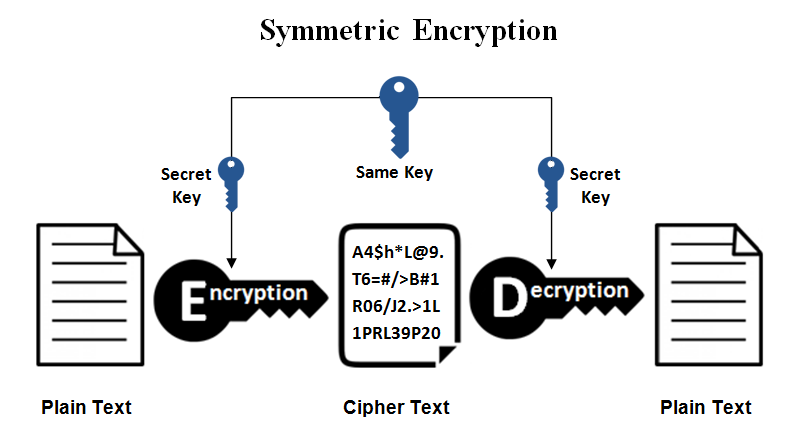
\includegraphics[scale=.27]{../pics/sym_crypto.png}}
    %             &
    %             \fbox{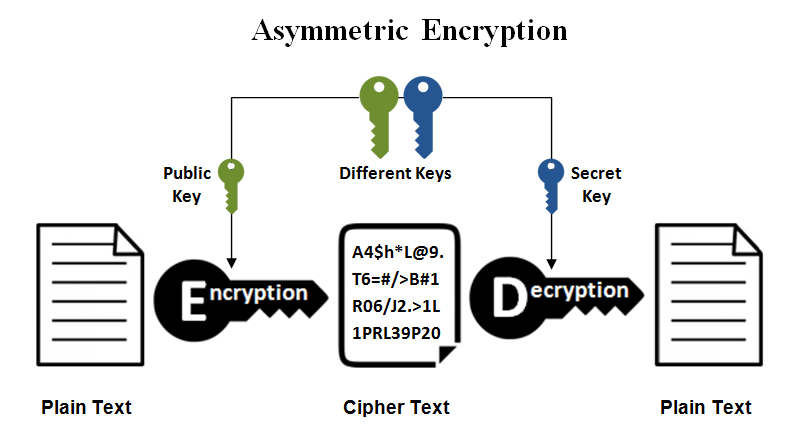
\includegraphics[scale=.27]{../pics/asym_crypto.png}}
    %             \vspace{3pt}
    %             \\
    %             Chiffre de César, AES, ...
    %             & RSA
    %         \end{tabular}
    %     \end{center}
    % \end{frame}

    \begin{frame}
        \frametitle{RSA}

        \begin{center}
            \fbox{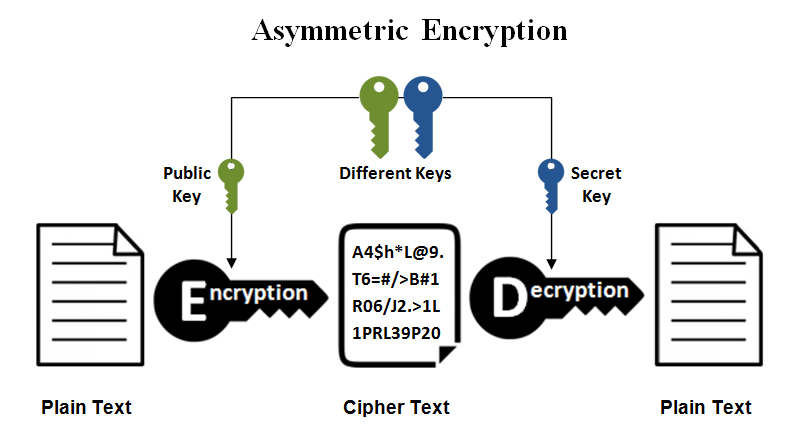
\includegraphics[scale=.4]{../pics/asym_crypto.png}}

            \vspace{6pt}
            
            Utilisation : HTTPS, cartes bancaires, ...
        \end{center}
    \end{frame}

    \begin{frame}
        \frametitle{Plan}

        \begin{multicols}{2}
            \tableofcontents
        \end{multicols}
    \end{frame}

    \begin{frame}
        \frametitle{Problématique / Objectifs}

        \begin{block}{Problématique}
            Pourquoi l'algorithme RSA est-il utilisé alors qu'il existe des attaques sur cet algorithme ?
        \end{block}

        \uncover<2->{
            \begin{block}{Objectifs}
                \begin{enumerate}
                    \item<2-> Implémentation de l'algorithme RSA (version naïve, et avec un schéma de remplissage) ;

                    \item<3-> \'Etude et implémentation d'attaques sur RSA ;

                    \item<4-> Montrer que l'implémentation de RSA doit être faite avec précaution.
                \end{enumerate}
            \end{block}
        }
    \end{frame}

    \section{Bases de RSA}
    % \subsection{Principe}

    \begin{frame}
        \frametitle{Bases de RSA}

        \begin{block}{\'Etapes de l'utilisation de RSA}
            \begin{enumerate}
                \item Génération des clés ;
            
                \item<2-> Chiffrement ;
            
                \item<3-> Déchiffrement.
            \end{enumerate}
        \end{block}
    \end{frame}

    \begin{frame}
        \frametitle{Génération des clés}

        \begin{itemize}
            \item<1-> Alice choisit $p, q$ deux grands nombres premiers.

            \item<2-> Le \emph{module de chiffrement} est $n = pq$.

            \item<3-> On note $\varphi = \varPhi(n) = (p - 1)(q - 1)$

            \item<4-> Alice choisi $e \in \nset 3 {\varphi - 1}$ premier avec $\varphi$, appelé \emph{exposant de chiffrement}

            \item<5-> Alice calcule $d \equiv e^{-1}\ [\varphi]$, appelé \emph{exposant de déchiffrement}

            \vspace{12pt}

            \item<6-> Clé publique : $(e, n)$
            \item<6-> Clé privée : $(d, n)$
        \end{itemize}
    \end{frame}

    \begin{frame}
        \frametitle{Chiffrement / Déchiffrement}

        Soit $m \in \nset 0 {n - 1}$.

        \uncover<2->{
            \begin{block}{Chiffrement}
                On chiffre $m$ par
                \[
                    c \equiv m^e\ [n]
                \]
            \end{block}
        }

        \uncover<3->{
            \begin{block}{Déchiffrement}
                Pour déchiffrer $c$ :
                \[
                    m \equiv c^d\ [n]
                \]
            \end{block}
        }

        \uncover<3->{Correction : $c^d \equiv m^{ed} \equiv m^{k\varphi + 1} \equiv m\ [n]$ par le théorème d'\textsc{Euler}.}
    \end{frame}

    \section{Attaques}
    \subsection{Premières attaques}

    \begin{frame}
        \frametitle{Propriété multiplicative}

        \begin{block}{Propriété :}
            On a :
            \[
                \lr{m_1 m_2}^e \equiv {m_1}^e {m_2}^e\ [n]
            \]
        \end{block}

        \vspace{12pt}
        
        \begin{itemize}
            \item<2-> Eve intercepte $c \equiv m^e\ [n]$.

            \item<3-> Soit $r \in \nset 1 {n - 1}\ |\ r \wedge n = 1$

             Soit $c' \equiv c r^e \equiv \lr{mr}^e\ [n]$

            \item<4-> Elle demande à Alice de déchiffrer $c'$ $\rightarrow$ $m' \equiv {c'}^d\ [n]$

            \item<5-> Eve récupère le message : $m \equiv m' r^{-1}\ [n]$
        \end{itemize}
    \end{frame}

    \begin{frame}
        \frametitle{Factorisation de $n$ avec $\varphi$}

        On a :
        \[
            \begin{array}{cl}
                &
                \begin{cases}
                    n = pq
                    \\
                    \varphi = (p - 1)(q - 1)
                \end{cases}
                \vspace{6pt}
                \\
                \ssi
                &
                \begin{cases}
                    n = pq
                    \\
                    \varphi = pq -p -q + 1
                \end{cases}
                \vspace{6pt}
                \\
                \ssi
                &
                \begin{cases}
                    pq = n
                    \\
                    p + q = n - \varphi + 1
                \end{cases}
                \vspace{6pt}
                \\
                \ssi
                &
                p, q\ \text{solutions de} \quad x^2 - (n - \varphi + 1)x + n = 0
            \end{array}
        \]

        Il suffit donc de calculer les racines de \Emph{$x^2 - (n - \varphi + 1)x + n$}
    \end{frame}

    %TODO: add the large message attack ?

    \subsection{Attaque de Wiener}

    \begin{frame}
        \frametitle{Attaque de Wiener -- Notations}

        L'\Emph{attaque de Wiener} permet de récupérer la \Emph{\it clé privée} $(d, n)$ à partir de la \Emph{\it clé publique} $(e, n)$ sous certaines conditions :

        \vspace{12pt}
        
        \begin{itemize}
            \item<2-> $q < p < 2q$ ;

            % \item $\displaystyle d \in \left[ 1\ ;\ \dfrac 1 3 n^{\tfrac 1 4} \right[ \cap \N$ ;

            \item<3-> $d < \dfrac 1 3 n^{\tfrac 1 4}$.
        \end{itemize}
    \end{frame}

    \begin{frame}
        \frametitle{Idée}

        On peut montrer que sous ces conditions,
        \[
            \oboxed{
                \abs{\dfrac e n - \dfrac k d} \le \dfrac 1 {2d^2}
            }
            \qquad (1)
        \]

        Où $k = \dfrac{ed - 1}{\varphi}$.

        \begin{itemize}
            \item Donc $\dfrac e n$ est une \emph{approximation} de $\dfrac k d$

            \item On va pouvoir retrouver $k$ et $d$ à l'aide des \emph{fractions continues}.
        \end{itemize}
    \end{frame}

    \begin{frame}[allowframebreaks]
        \frametitle{Fractions continues}

        \begin{block}{Définition (\emph{fraction continue})}
            Une \emph{fraction continue} est une fraction du type :
            \[
                a_0 + \dfrac{1}{a_1 + \dfrac{1}{
                    \begin{array}{ll}
                        \ddots \!\!\!\!\!\!\!\!
                        \\
                        & a_{n - 1} + \dfrac 1 {a_n}
                    \end{array}
                }}
            \]

            où $a_0 \in \N$, et $\forall k \in \nset 1 n,\ a_k \in \N^*$.

            On la note $[a_0, \ldots, a_n]$.
        \end{block}

        \newpage

        \begin{block}{Définition (\emph{réduites})}
            Soit $f = [a_0, \ldots, a_n]$ une fraction continue.

            Soient :
            \[
                \begin{array}{cc}
                    % \lr{p_k}_{k \in \nset{-2}{n}}
                    \begin{cases}
                        p_{-2} = 0
                        \\
                        p_{-1} = 1
                        \\
                        p_k = a_k p_{k - 1} + p_{k - 2}
                    \end{cases}
                    &
                    % \lr{q_k}_{k \in \nset{-2}{n}}
                    \begin{cases}
                        q_{-2} = 1
                        \\
                        q_{-1} = 0
                        \\
                        q_k = a_k q_{k - 1} + q_{k - 2}
                    \end{cases}
                \end{array}
            \]

            Alors les \emph{réduites} de $f$ sont les fractions ($k \in \nset 0 n$) :
            \[
                \dfrac{p_k}{q_k}
            \]
        \end{block}

        \newpage

        % \begin{block}{Propriété} %This propriety is useless for wiener's attack.
        %     Soit $f = [a_0, \ldots, a_n]$ une fraction continue, et $\dfrac{p_k}{q_k}$ ses réduites.
        %
        %     Alors :
        %     \[
        %         \forall k \in \nset 0 n,\
        %         \dfrac{p_k}{q_k} = [a_0, \ldots, a_k]
        %     \]
        % \end{block}

        \begin{block}{Fraction continue d'un rationnel}
            Soient $(a, b) \in \Z \times \N^*$.

            On peut calculer la fraction continue de $\dfrac a b$ avec l'algorithme suivant :

        \end{block}
        \vspace{-10pt}
        % \lstinputlisting[language=Python, firstline=258, lastline=269]{../../modules/arithmetic.py}
        \lstinputlisting[language=Python, firstline=290, lastline=300]{../../modules/arithmetic.py}

        \begin{block}{Théorème}
            Soient $a, a' \in \Z$, et $b, b' \in \Z^*$ tels que
            \[
                \abs{\dfrac{a}{b} - \dfrac{a'}{b'}} < \dfrac{1}{2b^2}
            \]

            Alors $\dfrac a b$ est une réduite de $\dfrac{a'}{b'}$.
        \end{block}

        \vspace{12pt}
        
        $\rightarrow$ On déduit donc de $(1)$ que $\dfrac k d$ est une réduite de $\dfrac e n$.
    \end{frame}

    \begin{frame}
        \frametitle{Attaque de Wiener}

        \begin{itemize}
            \item<1-> On calcule les réduites de $\dfrac e n$, que l'on note $\dfrac{k_i}{d_i}$ ;

            \vspace{6pt}
            
            \item<2-> On calcule $\varphi_i = \dfrac{e \cdot d_i - 1}{k_i}$ ;

            \vspace{6pt}

            \item<3-> On essaye de factoriser $n$ avec $\varphi_i$.
        \end{itemize}
    \end{frame}

    \begin{frame} %TODO: improve this frame !
        \frametitle{Extension de l'attaque de Wiener}

        \begin{itemize}
            \item<1-> On considère un $d$ \Emph{très grand} : il va être "petit", négatif modulo $\varphi$.
            
            \item<2-> On prend $d$ tel que
            \[
                \varphi - d < \dfrac 1 3 n^{\tfrac 1 4}
            \]

            \item<3-> On pose $D = \varphi - d \equiv -d\ [\varphi]$

            \item<4-> $D$ satisfait les propriétés précédentes : on va pouvoir de nouveau réaliser l'attaque, avec
                \[
                    \varphi_i = \dfrac{e \cdot d_i\ \Emph{+}\ 1}{k_i}
                \]
        \end{itemize}
    \end{frame}

    \begin{frame}
        \frametitle{Résultats}

        \begin{center}
            \fbox{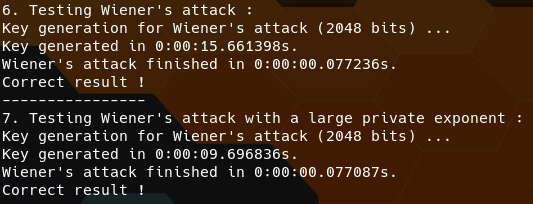
\includegraphics[scale=.7]{../screenshots/Wiener_Wiener_large_2048.png}}
        \end{center}
    \end{frame}

    \subsection{Attaque de Håstad}

    \begin{frame}
        \frametitle{Attaque de Håstad -- Notations}

        Alice envoie un même message $m$ à $p$ destinataires ayant le même exposant de chiffrement :
        \[
            \lr{S}
            \quad
            \left\{
            \begin{array}{rcl}
                c_1 & \equiv & m^e\ [n_1]
                \\
                    & \vdots
                \\
                c_p & \equiv & m^e\ [n_p]
            \end{array}
            \right.
        \]

        On suppose que tous les modules ont la même taille $s$ ($\forall k \in \nset 1 p,\ \log_2(n_k) \approx s$). Généralement, $s = 2048$.

        \vspace{12pt}
        
        L'\Emph{attaque de Håstad} va permettre de récupérer le message $m$ sous certaines conditions.
    \end{frame}

    \begin{frame}
        \frametitle{Solution au système}

        Par le théorème des restes chinois,
        \[
            (S)
            \ssi
            m^e \equiv \sum_{k = 1}^p c_k N_k M_k\ [N]
        \]

        où $\forall k \in \nset 1 p$ :
        \begin{itemize}
            \item $\displaystyle N = \prod_{k = 1}^p n_k$

            \item $\displaystyle N_k = \dfrac N {n_k}$

            \item $\displaystyle M_k \equiv {N_k}^{-1}\ [n_k]$
        \end{itemize}
    \end{frame}

    \begin{frame}
        \frametitle{Condition sur le nombre d'équations $p$}

        Pour retrouver le message, on a besoin que \Emph{$m^e < N$}.

        Or $\displaystyle N = \prod_{k = 1}^p n_k \approx 2^{sp}$

        Donc il faut que
        \[
            \oboxed{p > \dfrac e s \log_2(m)}
        \]

        $m \le 2^s - 1$, donc dans le cas général, $\oboxed{p > e}$.
    \end{frame}

    \begin{frame} %TODO: is this slide useful ?
        \frametitle{Résultats}

        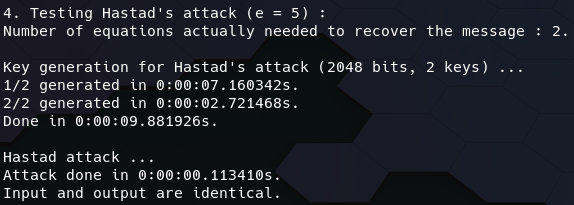
\includegraphics[scale=.55]{../screenshots/Hastad_2048.png}
        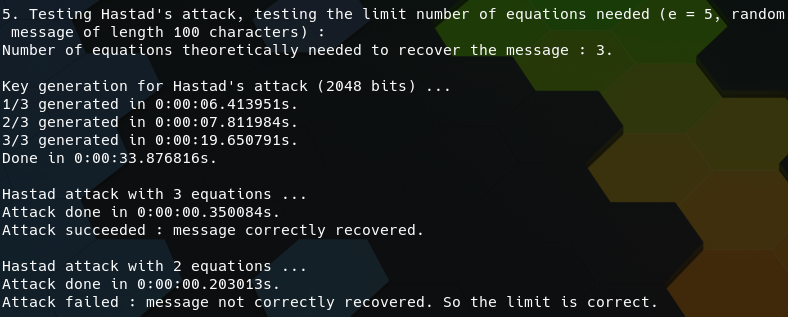
\includegraphics[scale=.5]{../screenshots/Hastad_test_limit_3.png}
    \end{frame}

    \section{Schéma de remplissage}
    \begin{frame}
        \frametitle{Nécessité d'un schéma de remplissage (\textit{padding scheme})}

        \begin{block}{Problèmes :}
            \begin{itemize}
                \item<1-> L'algorithme RSA est \Emph{déterministe} : tel quel, il n'est donc pas \emph{sémantiquement sûr}.
                
                \item<2-> Si $e$ et $m$ sont trop petits, on peut retrouver le message clair sans la clé privée (si $m^e < n$).
            \end{itemize}
        \end{block}

        \uncover<3->{$\rightarrow$ Il faut donc utiliser un schéma de remplissage.}
    \end{frame}

    \begin{frame}
        \frametitle{Le padding OAEP}

        \begin{center}
            \begin{tabular}{cp{100pt}}
                \fbox{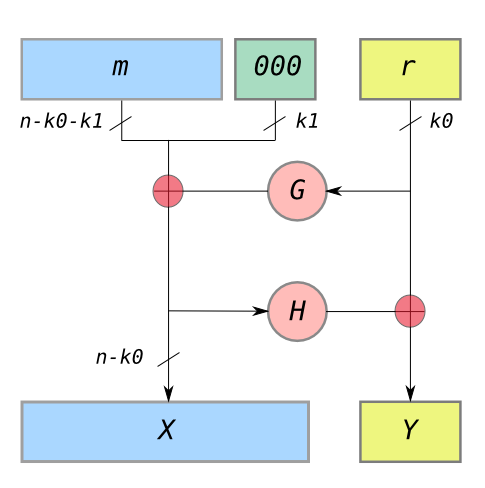
\includegraphics[scale=.4]{../pics/Oaep-diagram-20080305.png}}
                &
                \vspace{-150pt}
                \textbf{Encodage} :

                $X = m \overbrace{0 \cdots 0}^{k_1} \oplus G(r)$

                $Y = r \oplus H(X)$

                \vspace{12pt}
                
                \textbf{Décodage} :

                $r = Y \oplus H(X)$

                $m 0 \cdots 0 = X \oplus G(r)$
            \end{tabular}
        \end{center}

        \scriptsize{\url{https://fr.wikipedia.org/wiki/Optimal_Asymmetric_Encryption_Padding}}
    \end{frame}

    \section{Conclusion}

    \begin{frame}
        \frametitle{Conclusion}

        \begin{itemize}
            \item L'utilisation d'un \emph{padding} randomisé permet de se prémunir de l'attaque de \textsc{Håstad} ;

            \item Dans l'implémentation de la génération des clés, il faut vérifier que $d$ n'est pas dans les conditions de l'attaque de \textsc{Wiener}.
        \end{itemize}
    \end{frame}

    \begin{frame}
        \begin{center}
            \Large{\bf Merci pour votre attention}
        \end{center}
    \end{frame}

    \section{Annexes}

    \subsection{Correction de RSA}
    \begin{frame}
        \frametitle{Preuve de correction de l'algorithme RSA}

        \begin{block}{Théorème d'\textsc{Euler}}
            $\forall n \in \N^*$, $\forall a \in \nset 1 n\ |\ a \wedge n = 1$, on a :
            % Pour $n \in \N^*$, et $a \in \nset 1 n$ tel que $a \wedge n = 1$, on a :
            \[
                a^{\phi(n)} \equiv 1\ [n]
            \]
        \end{block}

        Comme $ed \equiv 1\ [\varphi],\quad \exists k \in \N\ |\ ed = k\varphi + 1$.

        \vspace{6pt}
        
        Donc on a :
        \[
            \orboxed{c^d}
            \equiv m^{ed}
            \equiv m^{k\varphi + 1}
            \equiv \olboxed{m}\ [n]
        \]
    \end{frame}

    \subsection{Preuve de l'attaque de Håstad}
    \begin{frame}
        \frametitle{Théorème des restes chinois}

        \begin{block}{Théorème des restes chinois :}
            Soient $p \in \N^*$ et $\lr{n_k}_{k \in \nset 1 p} \in \lr{\N^* \setminus \set 1}^p$ tels que
            \[
                \forall i, j \in \nset 1 p,\ i \neq j \Rightarrow n_i \wedge n_j = 1
            \]

            Avec $\displaystyle N = \prod_{k = 1}^p n_k$, on a que :
            \[
                \begin{array}{ccccc}
                    \psi & : & \Z / N\Z & \longrightarrow & \displaystyle \prod_{k = 1}^p \Z / n_k\Z
                    \\
                    && cl_N(x) & \longmapsto & \lr{cl_{n_1}(x), \ldots, cl_{n_p}(x)}
                \end{array}
            \]

            est un isomorphisme d'anneaux.
        \end{block}

        %TODO: put the proof in annexes ?
    \end{frame}

    \begin{frame}[allowframebreaks]
        \frametitle{Preuve de l'attaque de Håstad}

        On détermine $\psi^{-1}$ :
        \[
            \begin{array}{cl}
                & \psi^{-1}((cl_{a_1}(c_1), \ldots, cl_{a_n}(c_n)))
                \\
                =& \displaystyle
                \psi^{-1}\!\lr{\sum_{k = 1}^n c_k \lr{cl_{a_1}(0), \ldots, cl_{a_{k - 1}}(0), cl_{a_k}(1), cl_{a_{k + 1}}(0), \ldots, cl_{a_n}(0)}}
                \\
                =& \displaystyle
                \sum_{k = 1}^n c_k \underbrace{\psi^{-1} \lr{cl_{a_1}(0), \ldots, cl_{a_{k - 1}}(0), cl_{a_k}(1), cl_{a_{k + 1}}(0), \ldots, cl_{a_n}(0)}}_{cl_a(m_k)}
                \\
                =& \displaystyle \sum_{k = 0}^n c_k cl_a(m_k)
            \end{array}
        \]
    
        Il suffit de trouver des $m_k$ qui conviennent, c'est à dire tels que :
        \[
            \forall k \in \nset 1 n,\
            \begin{cases}
                m_k \in \Z
                \\
                \forall i \in \nset 1 n \setminus \set k,\
                m_k \equiv 0\ [a_i]
                \\
                m_k \equiv 1\ [a_k]
            \end{cases}
        \]
    
        Soit $A = \displaystyle \prod_{k = 1}^n a_k$, et $\forall k \in \nset 1 n$, $A_k = \dfrac{A}{a_k}$
    
        Comme les $a_k$ sont deux à deux premiers entre eux, $\forall k \in \nset 1 n,\ A_k \wedge a_k = 1$, donc avec le théorème de \textsc{Bézout} :
        \[
            \exists B_k, b_k \in \Z\ |\
            A_k B_k + a_k b_k = 1
        \]
        ($B_k \equiv \lr{A_k}^{-1}\ [a_k]$)
    
        \vspace{6pt}
    
        Soient $\forall k \in \nset 1 n,\ m_k = A_k B_k \in \Z$.
    
        \vspace{6pt}
    
        On a, $\forall k \in \nset 1 n$ :
        \[
            m_k \equiv A_k B_k \equiv 1 - a_k b_k \equiv 1\ [a_k]
        \]
    
        et $\forall i \in \nset 1 n \setminus \set k$ :
        \[
            m_k \equiv A_k B_k \equiv 0\ [a_i]
        \]
        car $a_i | A_k$.
    
        \vspace{12pt}
    
        Donc finalement :
        \[
            \psi^{-1}\lr{cl_{a_1}(c_1), \ldots, cl_{a_n}(c_n)}
            =
            \sum_{k = 1}^n c_k cl_a(A_k B_k)
        \]
    \end{frame}

    \subsection{Preuve de l'attaque de Wiener}
    \begin{frame}[allowframebreaks]
        \frametitle{Preuve de l'attaque de Wiener}

        Comme $ed \equiv 1\ [\varphi],\ \exists k \in \N\ |\ ed - k\varphi = 1$, donc :
        \[
            \begin{array}{rc}
                & \dfrac{ed - k \varphi}{d\varphi} = \dfrac{1}{d\varphi}
                \vspace{6pt}
                \\
                \Rightarrow&
                \dfrac e \varphi - \dfrac k d = \dfrac 1 {d \varphi}
                \vspace{6pt}
                \\
                \Rightarrow&
                \abs{\dfrac e \varphi - \dfrac k d} = \dfrac 1 {d \varphi}
            \end{array}
        \]
        
        Donc $\dfrac k d$ est une approximation de $\dfrac e \varphi$.
        
        On peut essayer d'approximer $\varphi$ avec $n$ :
        \[
            \varphi = \phi(n) = (p - 1)(q - 1) = n - p - q + 1
        \]
        
        Comme
        $
            \begin{cases}
                p < 2q
                \\
                q < p
            \end{cases}
        $
        (par hypothèse), on a :
        \[
            \begin{cases}
                p + q < 3q
                \\
                q^2 < pq = n
            \end{cases}
            \Rightarrow
            \begin{cases}
                p + q < 3q
                \\
                q < \sqrt n
            \end{cases}
            \Rightarrow
            p + q < 3\sqrt n
            \Rightarrow p + q - 1 < 3\sqrt n
        \]
        Donc $\abs{n - \varphi} = \abs{p + q - 1} < 3\sqrt n$.
        
        \vspace{12pt}
        
        On a ensuite :
        
        \[
            \begin{array}{rcl}
                \abs{\dfrac e n - \dfrac k d}
                &=& \abs{\dfrac{ed - nk}{nd}}
                \vspace{6pt}
                \\
                &=& \abs{\dfrac{ed - k\varphi + k\varphi - nk}{nd}}
                \vspace{6pt}
                \\
                &=& \abs{\dfrac{1 - k(n - \varphi)}{nd}}
                \vspace{6pt}
                \\
                &<& \dfrac{1 + \abs{k(n - \varphi)}}{\abs{nd}}
                \vspace{6pt}
                \\
                &\le& \abs{\dfrac{k(n - \varphi)}{nd}}
                \le \abs{\dfrac{3k\sqrt{n}}{nd}}
                = \dfrac{3k}{d\sqrt n}.
            \end{array}
        \]
        
        Ensuite, $k \varphi = ed - 1 < ed$ et $e < \varphi$, donc $k < \dfrac{e}{\varphi}d < d$, donc :
        \[
            k < d < \tfrac 1 3 n^{\frac 1 4}
            \ \Rightarrow\
            \dfrac k d < 1 < \dfrac{n^{\frac 1 4}}{3d}
        \]
        
        Donc :
        \[
            \begin{array}{rcl}
                \abs{\dfrac e n - \dfrac k d}
                &\le&
                \dfrac k d \dfrac{3}{\sqrt n}
                \vspace{6pt}
                \\
                &\le& \dfrac{n^{\frac 1 4}}{3d} \dfrac{3}{\sqrt n}
                \vspace{6pt}
                \\
                &=& \dfrac{1}{d n^{\frac 1 4}}
            \end{array}
        \]
        
        Et :
        \[
            2d^2 < \dfrac 2 3 dn^{\frac 1 4} < dn^{\frac 1 4}
            \ \Rightarrow\
            \dfrac 3 {2d n^{\frac 1 4}} < \dfrac 1 {2d^2}
        \]
        
        D'où :
        \[
            \oboxed{
            \abs{\dfrac e n - \dfrac k d}
            \le \dfrac{1}{dn^{\frac 1 4}}
            \le \dfrac{1}{2d^2}
            }
        \]
    \end{frame}

    \subsection{Structure du code}

    \begin{frame}
        \frametitle{Structure du code}
        \begin{center}
            \scalebox{.75}{
                \begin{forest}
                    for tree={
                        font=\sffamily,
                        text=black,
                        % text width=2cm,
                        % minimum height=0.75cm,
                        % if level=0
                        % {fill=ff4500}
                        % {draw=black},
                        rounded corners=4pt,
                        grow'=0,
                        child anchor=west,
                        parent anchor=south,
                        anchor=west,
                        calign=first,
                        edge={ff4500, rounded corners=1pt, line width=1pt},
                        edge path={
                            \noexpand\path [draw, \forestoption{edge}]
                            (!u.south west) +(0pt,0) |- (.child anchor)\forestoption{edge label};
                        },
                        before typesetting nodes={
                            if n=1
                            {insert before={[,phantom]}}
                            {}
                        },
                        fit=band,
                        s sep=8pt,
                        before computing xy={l=15pt},
                    }
                    [
                        [LICENCE]
                        [README.md]
                        [main.py]
                        [\textcolor{00f}{modules}
                            [arithmetic.py]
                            [base.py]
                            [RSA\_attacks.py]
                            [RSA.py]
                            [test\_attacks.py]
                            [tests.py]
                        ]
                    ]
                \end{forest}
            }
        \end{center}
    \end{frame}

    \subsection{Code}
    % \subsubsection{main.py}
    \begin{frame}[allowframebreaks]
        \frametitle{\texttt{main.py}}

        \lstinputlisting[language=Python]{../../main.py}
    \end{frame}

    % \subsubsection{arithmetic.py}
    \begin{frame}[allowframebreaks]
        \frametitle{\texttt{arithmetic.py}}

        \lstinputlisting[language=Python]{../../modules/arithmetic.py}
    \end{frame}

    % \subsubsection{base.py}
    \begin{frame}[allowframebreaks]
        \frametitle{\texttt{base.py}}

        \lstinputlisting[language=Python]{../../modules/base.py}
    \end{frame}

    % \subsubsection{RSA.py}
    \begin{frame}[allowframebreaks]
        \frametitle{\texttt{RSA.py}}

        \lstinputlisting[language=Python]{../../modules/RSA.py}
    \end{frame}

    % \subsubsection{RSA\_attacks.py}
    \begin{frame}[allowframebreaks]
        \frametitle{\texttt{RSA\_attacks.py}}

        \lstinputlisting[language=Python]{../../modules/RSA_attacks.py}
    \end{frame}

    % \subsubsection{test\_attacks.py}
    \begin{frame}[allowframebreaks]
        \frametitle{\texttt{test\_attacks.py}}

        \lstinputlisting[language=Python]{../../modules/test_attacks.py}
    \end{frame}

    % \subsubsection{tests.py}
    \begin{frame}[allowframebreaks]
        \frametitle{\texttt{tests.py}}

        \lstinputlisting[language=Python]{../../modules/tests.py}
    \end{frame}

\end{document}
